% Created 2024-06-24 Mon 14:26
% Intended LaTeX compiler: xelatex
\documentclass[11pt]{article}
\usepackage{hyperref}
% TIPS
% \substack{a\\b} for multiple lines text





% pdfplots will load xolor automatically without option
\usepackage[dvipsnames]{xcolor}

\usepackage{forest}
% two-line text in node by [two \\ lines]
% \begin{forest} qtree, [..] \end{forest}
\forestset{
  qtree/.style={
    baseline,
    for tree={
      parent anchor=south,
      child anchor=north,
      align=center,
      inner sep=1pt,
    }}}
%\usepackage{flexisym}
% load order of mathtools and mathabx, otherwise conflict overbrace

\usepackage{mathtools}
%\usepackage{fourier}
\usepackage{pgfplots}
\usepackage{amsthm, mathabx,  amsmath, commath}
\usepackage{amsfonts}

\usepackage{empheq}
\usepackage{tikz}
\usetikzlibrary{arrows.meta}
\usepackage[most]{tcolorbox}

\newtheorem{theorem}{Theorem}[section]
\newtheorem{definition}{Definition}[section]
\newtheorem{corollary}{Corollary}[section]
\newtheorem{example}{Example}[section]
\newtheorem{lemma}{Lemma}[section]
\newtheorem{proposition}{Proposition}[section]

\newcommand{\bl}[1] {\boldsymbol{#1}}
\newcommand{\Wt}[1] {\stackrel{\sim}{\smash{#1}\rule{0pt}{1.1ex}}}
\newcommand{\wt}[1] {\widetilde{#1}}


%For boxed texts in align, use Aboxed{}
%otherwise use boxed{}

\DeclareMathSymbol{\widehatsym}{\mathord}{largesymbols}{"62}
\newcommand\lowerwidehatsym{%
  \text{\smash{\raisebox{-1.3ex}{%
    $\widehatsym$}}}}
\newcommand\fixwidehat[1]{%
  \mathchoice
    {\accentset{\displaystyle\lowerwidehatsym}{#1}}
    {\accentset{\textstyle\lowerwidehatsym}{#1}}
    {\accentset{\scriptstyle\lowerwidehatsym}{#1}}
    {\accentset{\scriptscriptstyle\lowerwidehatsym}{#1}}
}

\usepackage{graphicx}
    
% text on arrow for xRightarrow
\makeatletter
%\newcommand{\xRightarrow}[2][]{\ext@arrow 0359\Rightarrowfill@{#1}{#2}}
\makeatother


\def \bx {\boldsymbol{x}}
\def \ba {\boldsymbol{a}}
\def \bI {\boldsymbol{I}}
\def \bt {\boldsymbol{t}}
\def \bb {\boldsymbol{b}}
\def \bA {\boldsymbol{A}}
\def \bX {\boldsymbol{X}}
\def \bu {\boldsymbol{u}}
\def \bS {\boldsymbol{S}}
\def \bZ {\boldsymbol{Z}}
\def \bz {\boldsymbol{z}}
\def \by {\boldsymbol{y}}
\def \bw {\boldsymbol{w}}
\def \bT {\boldsymbol{T}}
\def \bS {\boldsymbol{S}}
\def \bm {\boldsymbol{m}}
\def \bW {\boldsymbol{W}}
\def \bY {\boldsymbol{Y}}
\def \bH {\boldsymbol{H}}
\def \blambda {\boldsymbol{\lambda}}
\def \bPhi {\boldsymbol{\Phi}}
\def \btheta {\boldsymbol{\theta}}
\def \bmu {\boldsymbol{\mu}}
\def \bphi {\boldsymbol{\phi}}
\def \bSigma {\boldsymbol{\Sigma}}
\def \lb {\left\{}
\def \rb {\right\}}
\def \caln {\mathcal{N}}
\def \dissum {\displaystyle\Sigma}
\def \dispro {\displaystyle\prod}
\def \E {\mathbb{E}}
\def \Q {\mathbb{Q}}
\def \V {\mathbb{V}}
\def \R {\mathbb{R}}
\def \calq {\mathcal{Q}}
\def \calg {\mathcal{G}}
\def \caln {\mathcal{N}}
\def \calr {\mathcal{R}}
\def \calm {\mathcal{M}}
\def \calc {\mathcal{C}}
\def \bcup {\bigcup}

\graphicspath{{../../books/}}
\DeclareMathOperator{\flag}{\texttt{flag}}
\DeclareMathOperator{\victim}{\texttt{victim}}
\DeclareMathOperator{\tlevel}{\texttt{level}}
\makeindex

%% ox-latex features:
%   !announce-start, !guess-pollyglossia, !guess-babel, !guess-inputenc, caption,
%   underline, image, !announce-end.

\usepackage{capt-of}

\usepackage[normalem]{ulem}

\usepackage{graphicx}

%% end ox-latex features


\author{Many}
\date{\today}
\title{The Art of Multiprocessor Programming}
\hypersetup{
 pdfauthor={Many},
 pdftitle={The Art of Multiprocessor Programming},
 pdfkeywords={},
 pdfsubject={},
 pdfcreator={Emacs 29.1 (Org mode 9.7-pre)}, 
 pdflang={English}}
\begin{document}

\maketitle
\tableofcontents

\section{Mutual exclusion}
\label{sec:org8ca5ae0}
\subsection{Critical sections}
\label{sec:org6d321ca}
A good \texttt{Lock} algorithm should satisfy:
\begin{itemize}
\item \textbf{Mutual exclusion}: At most one thread holds the lock at any time.
\item \textbf{Freedom from deadlock}: If a thread is attempting to acquire or release the lock, then eventually
some thread acquires or relases the lock. If a thread calls \texttt{lock()} and never returns, then other
threads \uline{must complete an infinite number of critical sections} \wu{(different from normal deadlocks we counter)}.
\item \textbf{Freedom from starvation}: Every thread that attempts to acquire or release the lock eventually succeeds.
\end{itemize}
\subsection{The Peterson lock}
\label{sec:org97e7637}
\begin{listing}[htbp]
\begin{minted}[]{java}
class Peterson implements Lock {
    // thread-local index, 0 or 1
    private boolean[] flag = new boolean[2];
    private int victim;
    public void lock() {
        int i = ThreadID.get();
        int j = 1 - i;
        flag[i] = true;                   // I’m interested
        victim = i;                       // you go first
        while (flag[j] && victim == i) {} // wait
    }
    public void unlock() {
        int i = ThreadID.get();
        flag[i] = false;                  // I’m not interested
    }
}
\end{minted}
\caption{\label{}Pseudocode for the \texttt{Peterson} lock algorithm}
\end{listing}

\begin{lemma}[]
The \texttt{Peterson} lock algorithm satisfies mutual exclusion
\end{lemma}

\begin{proof}
Suppose not. Consider the last executions of the \texttt{lock()} method by threads \(A\) and \(B\).
\begin{align*}
&write_i(\flag[i]=true)\to write_i(\victim=i)\\&\quad\to read_i(\flag[j])\to read_i(\victim)\to CS_i
\end{align*}
Suppose \(A\) was the last thread to write to the \texttt{victim} field, then \(A\) observed \texttt{victim} to be
\(A\). Since \(A\) nevertheless entered its critical section, it must have observed \(\flag[B]\) to be
\emph{false}, so we have
\begin{equation*}
write_A(\victim=A)\to read_A(\flag[B]==false)
\end{equation*}
and
\begin{align*}
&write_B(\flag[B]=true)\to write_B(\victim=B)\\&\quad\to write_A(\victim=A)\to read_A(\flag[B]==false)
\end{align*}
A contradiction.
\end{proof}

\begin{lemma}[]
The \texttt{Peterson} lock algorithm is starvation-free.
\end{lemma}

\begin{proof}
Suppose not, so some thread runs forever in the \texttt{lock()} method. Suppose that it is \(A\).

If \(B\) is repeatedly entering and leaving its critical section, then \(B\) sets \texttt{victim} to \(B\)
before it reenters the critical section. Therefore \(A\) must eventually return from the \texttt{lock()}.

So \(B\) is also stuck in its \texttt{lock()} method. But \texttt{victim} cannot be both \(A\) and \(B\).
\end{proof}

\begin{corollary}[]
The \texttt{Peterson} lock algorithm is deadlock-free.
\end{corollary}
\subsection{The filter lock}
\label{sec:org0facba8}
\begin{listing}[htbp]
\begin{minted}[]{java}
class Filter implements Lock {
    int[] level;
    int[] victim;
    public Filter(int n) {
        level = new int[n];
        victim = new int[n]; // use 1..n-1
        for (int i = 0; i < n; i++) {
            level[i] = 0;
        }
    }
    public void lock() {
        int me = ThreadID.get();
        for (int i = 1; i < n; i++) { // attempt to enter level i
            level[me] = i;
            victim[i] = me;
            // spin while conflicts exist
            while ((∃k != me) (level[k] >= i && victim[i] == me)) {};
        }
    }
    public void unlock() {
        int me = ThreadID.get();
        level[me] = 0;
    }
}
\end{minted}
\caption{\label{}Psudocode for the \texttt{Filter} lock algorithm}
\end{listing}

The \texttt{Filter} lock creates \(n-1\) \textbf{levels}, that a thread must traverse before acquiring the lock. Levels
satisfy two properties:
\begin{enumerate}
\item At least one thread trying to enter level \(l\) succeeds.
\item If more than one thread is trying to enter level \(l\), then at least one is blocked (i.e.,
continues to wait without entering that level).
\end{enumerate}

\begin{center}
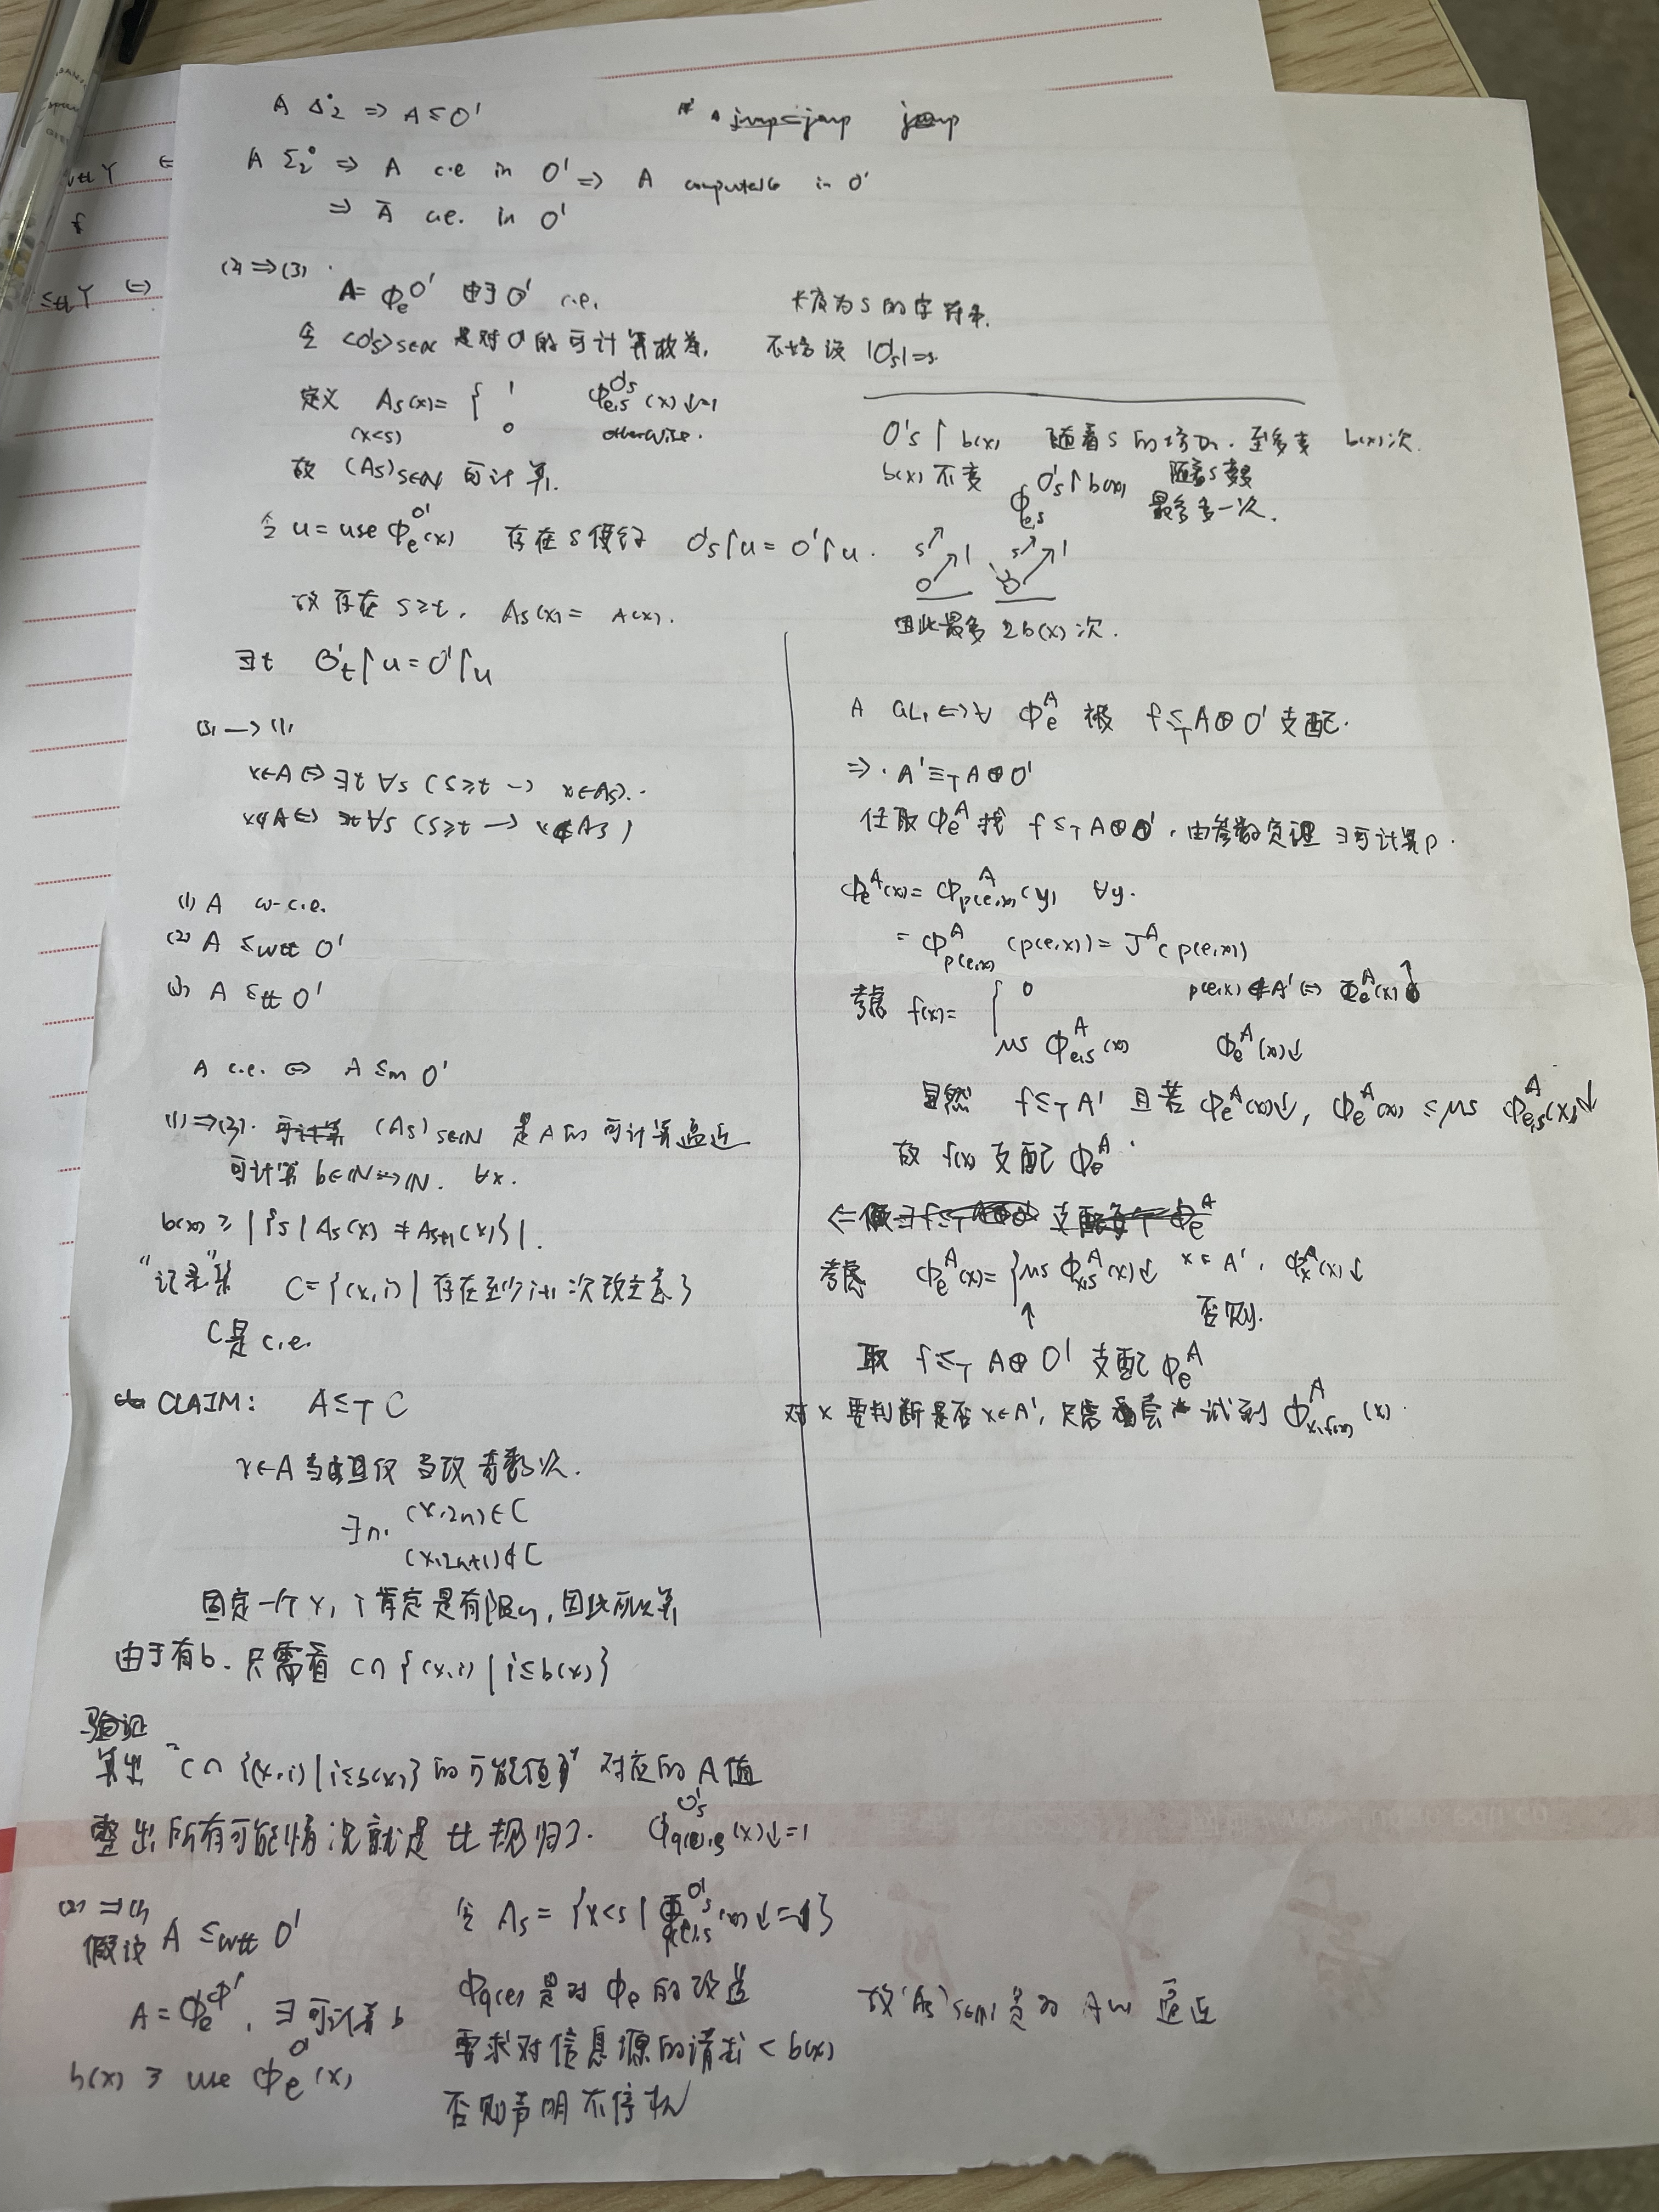
\includegraphics[width=.9\textwidth]{../images/ArtOfMulti/1.png}
\label{}
\end{center}
The value of \(\texttt{level}[A]\) indicates the highest level that thread \(A\) is trying to enter.

Initially, a thread \(A\) is at level 0. \(A\) \textbf{enters} level \(l>0\) when it completes the \texttt{while} loop
with \(\tlevel[A]=l\). \(A\) enters its critical section when it enters level \(n-1\). When \(A\)
leaves the critical section, it sets \(\tlevel[A]=0\).

\begin{lemma}[]
For \(j\) between \(0\) and \(n-1\), at most \(n-j\) threads have entered level \(j\) (and not
subsequently exited the critical section).
\end{lemma}

\begin{proof}
Induction. IH implies that at most \(n-j+1\) threads have entered level \(j-1\). Assume that \(n-j+1\)
threads have entered level \(j\). Because \(j\le n-1\), there must be at least two such threads
(\(n-j+1\ge 2\)).

Let \(A\) be the last thread to write \(\victim[j]\). \(A\) must have entered level \(j\) since
\(\victim[j]\) is written only by threads that have entered level \(j-1\), and, by the IH, every
thread that has entered level \(j-1\) has also entered level \(j\).

Let \(B\) be any thread other than \(A\) that has entered level \(j\). Inspecting the code, we see
that before \(B\) enters level \(j\), it first writes \(j\) to \(\tlevel[B]\) and then writes \(B\) to
\(\victim[j]\). Since \(A\) is the last to write \(\victim[j]\), we have
\begin{equation*}
write_B(\tlevel[B]=j)\to write_B(\victim[j])\to write_A(\victim[j]).
\end{equation*}
We also see that \(A\) reads \(\tlevel[B]\) after it writes to \(\victim[j]\), so
\begin{align*}
&write_B(\tlevel[B]=j)\to write_B(\victim[j])\\&\quad\to write_A(\victim[j])\to read_A(\tlevel[B]).
\end{align*}
Because \(B\) has entered level \(j\), every time \(A\) reads \(\tlevel[B]\), it observes a value
greater than or equal to \(j\), and since \(\victim[j]=A\), \(A\) couldn't completed its waiting loop.
\end{proof}

\begin{corollary}[]
The \texttt{Filter} lock algorithm satisfies mutual exclusion.
\end{corollary}

\begin{lemma}[]
The \texttt{Filter} lock algorithm is starvation-free.
\end{lemma}

\begin{proof}
We prove by induction on \(j\) that every thread that enters level \(n-j\) eventually enters and
leaves the critical section (assuming that it keeps taking steps and that every thread that enters the
critical section eventually leaves it). The base case, with \(j=1\), is trivial because level \(n-1\)
is the critical section.

For the induction step, we suppose that every thread that enters level \(n-j\) or higher eventually
enters and leaves the critical section, and show that every thread that enters level \(n-j-1\) does
too.

Suppose, for contradiction, that a thread \(A\) has entered level \(n-j-1\) and is stuck. By IH, it
never enters level \(n-j\), so it must be stuck at loop with \(\tlevel[A]=n-j\) and
\(\victim[n-j]=A\). After \(A\) writes \(\victim[n-j]\), no thread enters level \(n-j-1\).
Furthermore, any other thread \(B\) trying to enter level \(n-j\) will eventually succeed because
\(\victim[n-j]=A\neq B\), so eventually no threads other than \(A\) are trying to enter level \(n-j\).
Moreover, any thread that enters level \(n-j\) will, by IH, enter and leave the critical section,
setting its level to 0. In particular, after this point, \(\tlevel[B]<n-j\) for every thread \(B\)
other than \(A\), so \(A\) can enter level \(n-j\), a contradiction.
\end{proof}

\begin{corollary}[]
The \texttt{Filter} lock algorithm is deadlock-free.
\end{corollary}
\subsection{wefwef}
\label{sec:org5c03170}
\end{document}
